\documentclass[aspectratio=169,11pt]{beamer}

% Shared style (ib-tutorials.sty at the repo root).
\makeatletter\def\input@path{{./}{../}}\makeatother
\usepackage{ib-tutorials}

\usepackage[utf8]{inputenc}
\usepackage{amsmath,amssymb}
\usepackage{booktabs}
\usepackage{array}
\newcolumntype{L}[1]{>{\raggedright\arraybackslash}p{#1}}
\usepackage{graphicx}
\graphicspath{{../pictures/5-visit/}{pictures/5-visit/}}
\usepackage{xcolor}
\usepackage{listings}
\usepackage{tikz}
\usetikzlibrary{arrows.meta,positioning,shapes.geometric,fit,calc}
\usepackage{hyperref}

\newcommand{\sourcecredit}[1]{\vfill\begin{flushright}\tiny\textcolor{DarkGray}{#1}\end{flushright}}
\newcommand{\gui}[1]{\textsf{\textbf{#1}}}

\lstset{
  basicstyle=\ttfamily\scriptsize\color{BlackGray},
  keywordstyle=\color{NavyBlue}\bfseries,
  commentstyle=\color{DarkGray}\itshape,
  stringstyle=\color{OliveGreen},
  showstringspaces=false,
  columns=fullflexible,
  keepspaces=true,
  breaklines=true,
  breakindent=1em,
  frame=single,
  framerule=0.4pt,
  rulecolor=\color{LightGray},
  backgroundcolor=\color{LightGray!30},
  xleftmargin=0.25em,
  xrightmargin=0.25em
}
\lstdefinestyle{shell}{morecomment=[l]{\#}}
\lstdefinestyle{python}{morecomment=[l]{\#}}
\lstdefinestyle{tiny}{basicstyle=\ttfamily\tiny\color{BlackGray}}
\lstdefinestyle{pytiny}{morecomment=[l]{\#},basicstyle=\ttfamily\tiny\color{BlackGray}}

\title[VisIt: data analysis]{VisIt: data analysis}
\subtitle{Sampling, averaging and measuring: a box, queries frame by frame and through time, a pick through time, lineouts, the flow rate across a line, expressions, curves exported and read back; and a written record of how every number was made}
\author[Miller]{Laura A. Miller}
\institute[UArizona]{Department of Mathematics, University of Arizona}
\date{Using IB Software \textbullet\ Part V \textbullet\ Chapter 29}

\begin{document}

% 1
\begin{frame}[plain]
\maketutorialtitlepanel{%
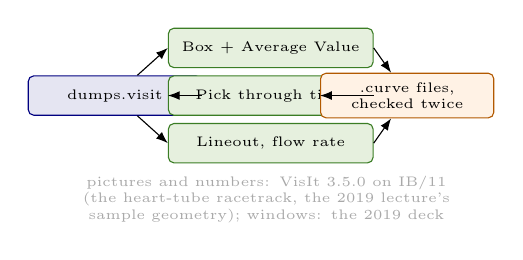
\begin{tikzpicture}[scale=0.55, every node/.style={font=\tiny}]
  \node[draw=NavyBlue,fill=NavyBlue!10,rounded corners=2pt,minimum width=2.2cm,minimum height=0.5cm] (d) at (0,0) {\code{dumps.visit}};
  \node[draw=OliveGreen,fill=OliveGreen!10,rounded corners=2pt,minimum width=2.6cm,minimum height=0.5cm,align=center] (b) at (3.6,1.1) {Box + Average Value};
  \node[draw=OliveGreen,fill=OliveGreen!10,rounded corners=2pt,minimum width=2.6cm,minimum height=0.5cm,align=center] (p) at (3.6,0) {Pick through time};
  \node[draw=OliveGreen,fill=OliveGreen!10,rounded corners=2pt,minimum width=2.6cm,minimum height=0.5cm,align=center] (l) at (3.6,-1.1) {Lineout, flow rate};
  \node[draw=orange!70!black,fill=orange!10,rounded corners=2pt,minimum width=2.2cm,minimum height=0.5cm,align=center] (c) at (6.75,0) {\code{.curve} files,\\checked twice};
  \foreach \t in {b,p,l} {\draw[-{Latex[length=1.5mm]}] (d) -- (\t.west); \draw[-{Latex[length=1.5mm]}] (\t.east) -- (c);}
  \node[text=DarkGray,align=center,text width=5.2cm] at (3.5,-2.4) {pictures and numbers: VisIt 3.5.0 on IB/11 (the heart-tube racetrack, the 2019 lecture's sample geometry); windows: the 2019 deck};
\end{tikzpicture}}
\end{frame}

% 2
\begin{frame}{Learning goals}
\label{fr:goals}
\footnotesize By the end of this chapter you should be able to:
\begin{itemize}
  \item Keep a written record of an analysis that someone else could repeat: a protocol, a data sheet per run, a report.
  \item Restrict a measurement to a box, and average a field over it, frame by frame and through time.
  \item Follow a variable through time at a point (a pick through time), and sample it along a line (a lineout).
  \item Turn a lineout into a flow rate, and check a flow rate on several lines.
  \item Export curves from VisIt and read them in Python, MATLAB or R.
  \item Check every number a second way, because some of VisIt's routes give different answers.
\end{itemize}
\begin{punchbox}
\small Every number in an analysis is a box, a point or a line, a query, and a time axis. Write all four down, and measure each number two ways.
\end{punchbox}
\end{frame}

% 3
\begin{frame}{Where this chapter comes from}
\label{fr:sources}
\scriptsize
\begin{itemize}
  \item \al{Lindsay Waldrop's VisIt guide}, ``Data analysis in VisIt'' (MATH 769; dated 16 February 2015 and written with VisIt 2.5.2 for IBAMR's output; quoted here from its 2017 version for IB2d's \code{.vtk} output): loading data, plots, movies, and a ``Data Analysis'' section: best practices for data analysis, restricting data capture with a box, Query and Query over time, a pick at a point through time, exporting curves (MATLAB, R).
  \item \al{``4 -- Visit Data Analysis -- Sampling and Time Queries''} (2019, 24 slides, ``Adapted from Lindsay Waldrop's Visit Tutorial''): ``the first of three lectures on how to extract information from data in visit'' (the GUI; export to MATLAB; Python on the cluster); the same recipes on a racetrack pumped by an elastic section, plus a lineout.
  \item \al{``Lecture 9: Sampling, averaging, and analyzing data in Visit''} (59 slides, ``Adapted from Lindsay Waldrop's and Nick Battista's Visit Tutorials''): slides 37--59 are the 2019 deck's text (its first 36 slides are chapters 26 and 27).
  \item \al{``3B -- Analyzing your IBFE simulation''} (2018), slides 12--16: a box above the corals, its average vertical flow through time, the curve in MATLAB.
\end{itemize}
\al{New here:} the 2019 sample data is IB/11's racetrack (next slides), so every recipe is redone on it in VisIt 3.5.0 and checked: the time query and the frame-by-frame query compared, the lineout turned into a flow rate on six lines round the loop, the curve files read in Python and in MATLAB/Octave (R's line given, not run), templates for the written record, and a script for all of it (\code{examples/analysis/visit\_queries.py}).
\end{frame}

% 4
\begin{frame}{Best practices first (Waldrop)}
\label{fr:practice}
\footnotesize
``As researchers, we are responsible for leaving a clear, understandable record of what we did to reach the conclusions in our papers \dots\ transparency and reproducibility are the ultimate goals of all scientific endeavors.''

\vspace{1mm}
A written \al{protocol} should include:
\begin{itemize}
  \item the coordinates of each box or position where data were collected or analysed, with a labelled figure;
  \item the method(s) by which the data were analysed (``were the data in the box averaged? was the max value found?'');
  \item step-by-step instructions for reproducing each output file, ``detailed enough that an undergraduate with a basic familiarity with VisIt could reproduce your plots without consulting you directly'';
  \item any plots, and the code (``documented appropriately'') for reproducing them.
\end{itemize}
And a \al{data sheet} in each simulation's folder: ``a clear, handy record of the parameters that the simulation used and any other identifying information''.
\sourcecredit{L. Waldrop, VisIt guide, ``Best Practices for Data Analysis''.}
\end{frame}

% 5
\begin{frame}{The analysis report, and general tips (Waldrop)}
\label{fr:tips}
\footnotesize
An \al{analysis report}: a condensed protocol (``what you would write in the Materials and Methods section of a paper''), any statistics so far, graphs with thorough captions, and rough notes on what you found; ``an excellent first draft of subsequent writing''.

\vspace{1mm}
General tips:
\begin{itemize}
  \item ``Err on the side of writing down too many details.'' ``Record as you go along.''
  \item ``Pick a clear naming convention and stick with it'': for a sweep, one folder per sweep and one subfolder per value (``Wosweep'' holding ``Wo10'', ``Wo0.5''), and a spreadsheet of where everything is.
  \item ``Leave a READ ME file in the first directory'': the study, the naming system, where the spreadsheet, the protocol and the report are, and which runs exist but were not used.
  \item ``Clean up old files and simulations as you go along.''
  \item ``Pretend like you won't remember anything in a week.''
\end{itemize}
\al{New:} \code{examples/analysis/templates/}: \code{analysis\_protocol.md}, \code{data\_sheet.md}, \code{analysis\_report.md}, each with this chapter's IB/11 analysis filled in as the example (the guide says examples ``should be included with these files''; none came with the copy used here).
\sourcecredit{L. Waldrop, VisIt guide, ``Best Practices for Data Analysis''.}
\end{frame}

% 6
\begin{frame}{The sample data is IB/11's racetrack}
\label{fr:data}
\begin{columns}[T]
\column{0.5\textwidth}
\footnotesize
The 2019 deck: ``The data was generated from a code where flow is driven through a racetrack through the pumping of an elastic section at the bottom of the track. The sides and the top of the racetrack are rigid. There is also a rigid box around the elastic part. If you plot markers, it will show passive tracers \dots\ If you plot \code{vp\_aforce} it will show the springs that drive the contraction.''

\vspace{1mm}
That is IB/11 (chapter 9b): the loop's centre lines at $y = \pm 0.15$, tube diameter $D = 0.1$, the elastic bottom section inside a rigid pericardium. The deck's box ($0 \le x \le 0.01$, $0.10 \le y \le 0.20$), point $(0, 0.15)$ and line $(0, 0.1)$--$(0, 0.2)$ all sit on the top vessel.
\column{0.48\textwidth}
\footnotesize
Here: the \code{TARGET\_VP} run of chapter 9b (suction by target points; IBAMR 0.19.0): 51 frames, $t = 0$ to $2$ s every $0.04$ s, 4 levels, finest $\Delta x = 1/512$; $\rho = 1000$, $\mu = 0.157$ (Wo $= 10$ at 1 Hz). The flow round the loop also uses \code{FORCE\_VP} (suction by an applied force, \code{Fmag\_vp} $= 0.25$).

\vspace{1mm}
IBAMR 0.19 writes the velocity only as the vector \code{U} (the 2019 menu had \code{U\_x}): define \code{U\_x = U[0]}, \code{U\_y = U[1]}, \code{speed = magnitude(U)} in \gui{Controls $\to$ Expressions} (chapter 26), which also avoids VisIt 3.5's trouble with its own \code{U\_magnitude} beside a plot from a second database (chapter 27).
\end{columns}
\sourcecredit{The 2019 deck, slide 3; \code{examples/IB/11-heart-tube-pump} and its README.}
\end{frame}

% 7
\begin{frame}{Where we measure}
\label{fr:map}
\begin{columns}[T]
\column{0.5\textwidth}
\centering
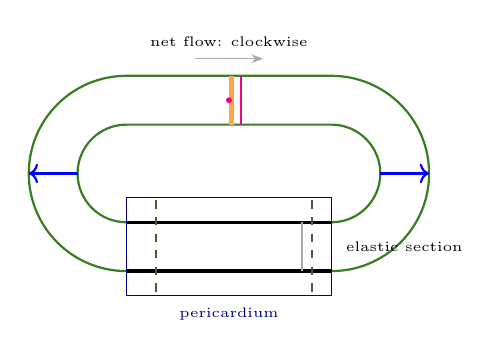
\begin{tikzpicture}[scale=6.2]
  \draw[OliveGreen,thick] (-0.21,0.2) -- (0.21,0.2) arc (90:-90:0.2) -- (-0.21,-0.2) arc (270:90:0.2);
  \draw[OliveGreen,thick] (-0.21,0.1) -- (0.21,0.1) arc (90:-90:0.1) -- (-0.21,-0.1) arc (270:90:0.1);
  \draw[black,very thick] (-0.21,-0.1) -- (0.21,-0.1); \draw[black,very thick] (-0.21,-0.2) -- (0.21,-0.2);
  \draw[NavyBlue] (-0.21,-0.05) rectangle (0.21,-0.25);
  \fill[orange!70] (0,0.1) rectangle (0.01,0.2);
  \fill[RubineRed] (0,0.15) circle (0.006);
  \draw[RubineRed,thick] (0.025,0.1) -- (0.025,0.2);
  \draw[blue,thick,->] (-0.31,0) -- (-0.41,0); \draw[blue,thick,->] (0.31,0) -- (0.41,0);
  \draw[DarkGray,thick] (0.15,-0.1) -- (0.15,-0.2);
  \draw[OliveGreen!60!black,thick,dashed] (0.17,-0.055) -- (0.17,-0.245); \draw[OliveGreen!60!black,thick,dashed] (-0.15,-0.055) -- (-0.15,-0.245);
  \draw[-{Stealth[length=1.5mm]},DarkGray] (-0.07,0.235) -- (0.07,0.235);
  \node[font=\tiny,anchor=south] at (0,0.24) {net flow: clockwise};
  \node[font=\tiny,text=NavyBlue,anchor=north] at (0,-0.255) {pericardium};
  \node[font=\tiny,anchor=west] at (0.22,-0.15) {elastic section};
\end{tikzpicture}
\column{0.48\textwidth}
\scriptsize
\begin{itemize}
  \item \textcolor{orange!80!black}{Box}: $0 \le x \le 0.01$, $0.10 \le y \le 0.20$, a stripe across the top vessel (the 2019 deck's).
  \item \textcolor{RubineRed}{Point} $(0, 0.15)$, the vessel's centre, and the \textcolor{RubineRed}{line} from $(0, 0.1)$ to $(0, 0.2)$ across it (drawn beside the box here; it lies on the box's edge).
  \item The flow rate round the loop on six lines: the top line, the two bends at $y = 0$ (\textcolor{blue}{blue}), the elastic section at $x = 0.15$ between the walls' rest positions (\textcolor{DarkGray}{grey}), and at $x = \pm 0.15$ across the whole pericardium (\textcolor{OliveGreen!60!black}{dashed}, drawn apart).
  \item Positive flow on every line: clockwise round the loop, $+x$ along the top.
\end{itemize}
\end{columns}
\sourcecredit{Drawn to scale from IB/11's generator (chapter 9b).}
\end{frame}

% 8
\begin{frame}{Restricting data capture with a box}
\label{fr:box}
\begin{columns}[T]
\column{0.35\textwidth}
\centering
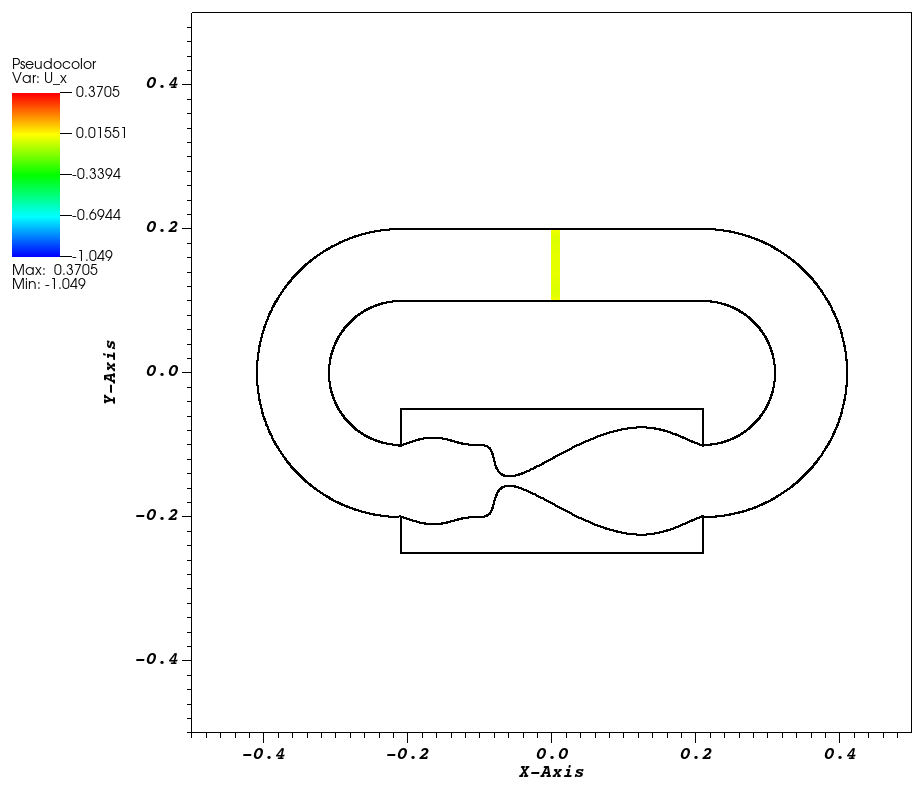
\includegraphics[width=\textwidth]{ch29-box.png}
\column{0.63\textwidth}
\scriptsize
``It is sometimes useful to restrict your data analysis to a very small part of your total graph \dots\ It doesn't matter how wide the box is, so long as you use the same box for every step of the analysis (and every simulation you analyze).''
\begin{itemize}
  \item ``Under the Plots section, you should see two check boxes labeled `Apply operators to all plots' and `Apply subset selections to all plots.' Uncheck both of these boxes.'' Then a Pseudocolor plot of \code{U\_x}, \gui{Operators $\to$ Selection $\to$ Box}, and the box's minimum and maximum $x$ and $y$ (the window also has $z$ fields, 0 to 1 by default, as the 2019 deck's window on its slide 9 already had: keep a range containing 0, chapter 28).
  \item Picture: \code{U\_x} only inside the box at $t = 2$ (one yellow: the colour bar keeps the whole field's range, $-1.05$ to $0.37$ m/s, while \code{U\_x} in the box runs from $-0.039$ to $0.003$), and the loop's points.
  \item \gui{Amount of cell in the range}: \gui{Some} keeps every cell that is partly inside or touches the box (here 7 $\times$ 52 cells of $1/512$ m: a column that only touches $x = 0$, and rows over 0.1016 m for the vessel's 0.1), \gui{All} only cells wholly inside (5 $\times$ 50). Here, on the four frames checked, \gui{Some} kept $0.0014$--$0.0018$ m$^2$ for the nominal $0.001$, changing as the grid regridded; \gui{All} $0.00088$--$0.00095$. Say which you used.
\end{itemize}
\end{columns}
\sourcecredit{The 2019 deck, slides 5--9 (the guide's 2017 version boxes a quarter of IB2d's rubber band; its 2015 original used $0 \le x \le 0.01$, $0.10 \le y \le 0.12$, where ``the vessel goes from about 0.10 to 0.12'' in its geometry). IB/11 \code{TARGET\_VP}, VisIt 3.5.0; areas from the 2D area query.}
\end{frame}

% 9
\begin{frame}{Query over time: the time axis}
\label{fr:qot}
\begin{columns}[T]
\column{0.42\textwidth}
\centering
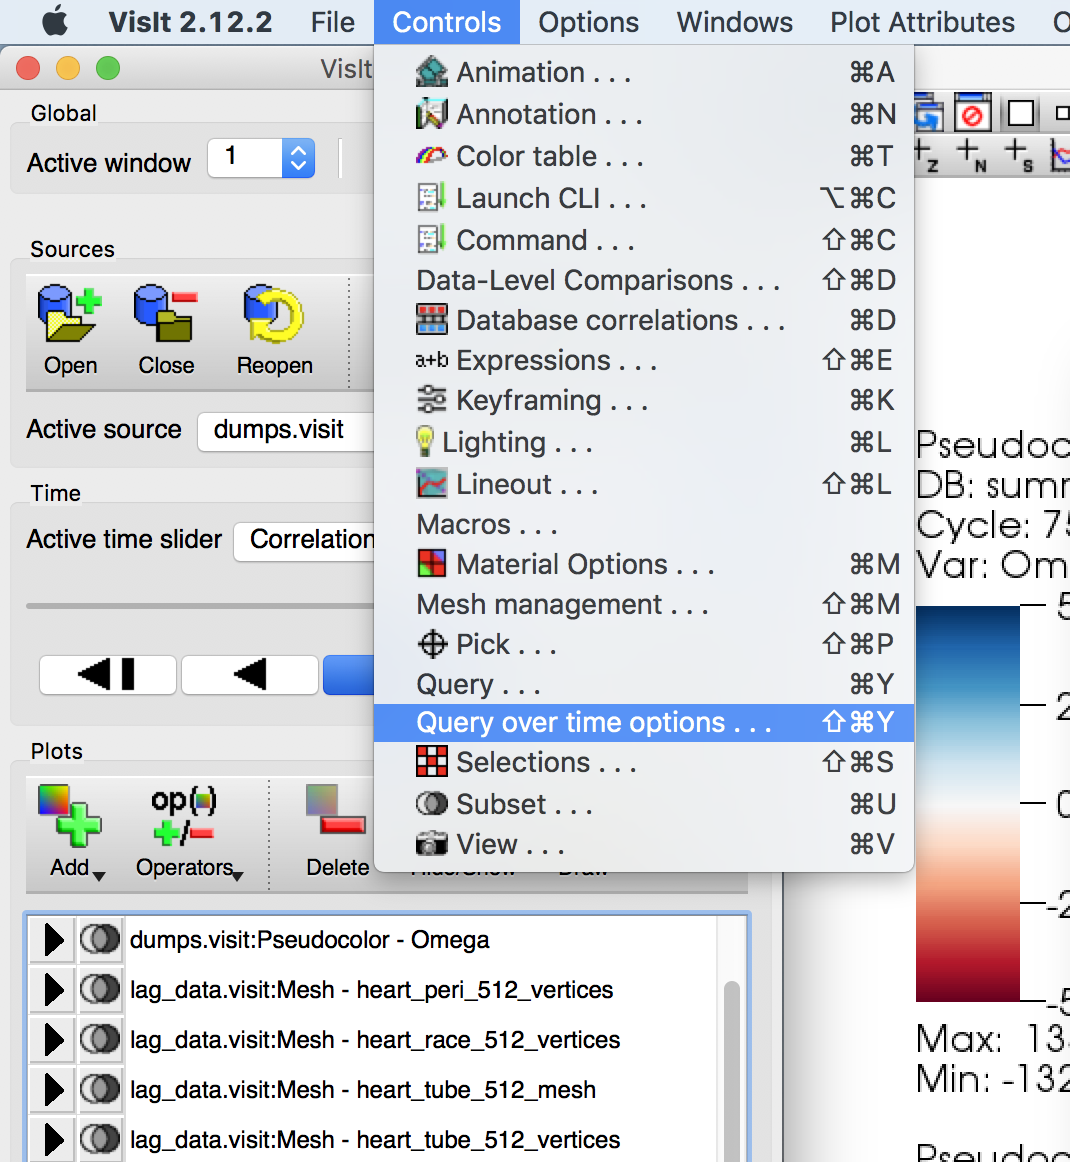
\includegraphics[width=0.95\textwidth]{ch29-2019-controls-menu.png}
\column{0.56\textwidth}
\scriptsize
``Before your first Query, you need to select `Query over time options\dots' right below Query \dots\ there will be a line of toggle buttons along the top with the options `Cycle, Time, Timestep.' Select `Time' and hit Apply.''
\begin{itemize}
  \item The choice is the curve's $x$-axis: the cycle (time-step number), the time, or the frame index. VisIt 3.5's default is still \gui{Cycle} (in a script: \code{GetQueryOverTimeAttributes().timeType}, with the values \code{Cycle}, \code{DTime}, \code{Timestep}).
  \item The same window says where the curve goes: \gui{Use 1st unused window or create new one} (ticked by default; window 2 here), or a \gui{Window \#} you give. The frames (start, end, stride) are chosen in the Query window (next slide's picture): the Query over time window lost them in 2011, though the 3.5 manual and \code{GetQueryOverTimeAttributes()} still list them.
  \item Queries that run through time in 3.5 include \gui{Average Value}, \gui{Variable Sum}, \gui{Weighted Variable Sum}, \gui{Min}, \gui{Max}, \gui{2D area}, \gui{Volume} and the two trajectory queries (\code{QueriesOverTime()} lists 20).
\end{itemize}
\end{columns}
\sourcecredit{Left: the 2019 deck, slide 11 (VisIt 2.12.2). VisIt 3.5.0: \code{QueriesOverTime()}, \code{GetQueryOverTimeAttributes()}, the window's source (\code{QvisQueryOverTimeWindow.C}).}
\end{frame}

% 10
\begin{frame}{Average Value through time}
\label{fr:avg}
\begin{columns}[T]
\column{0.4\textwidth}
\centering
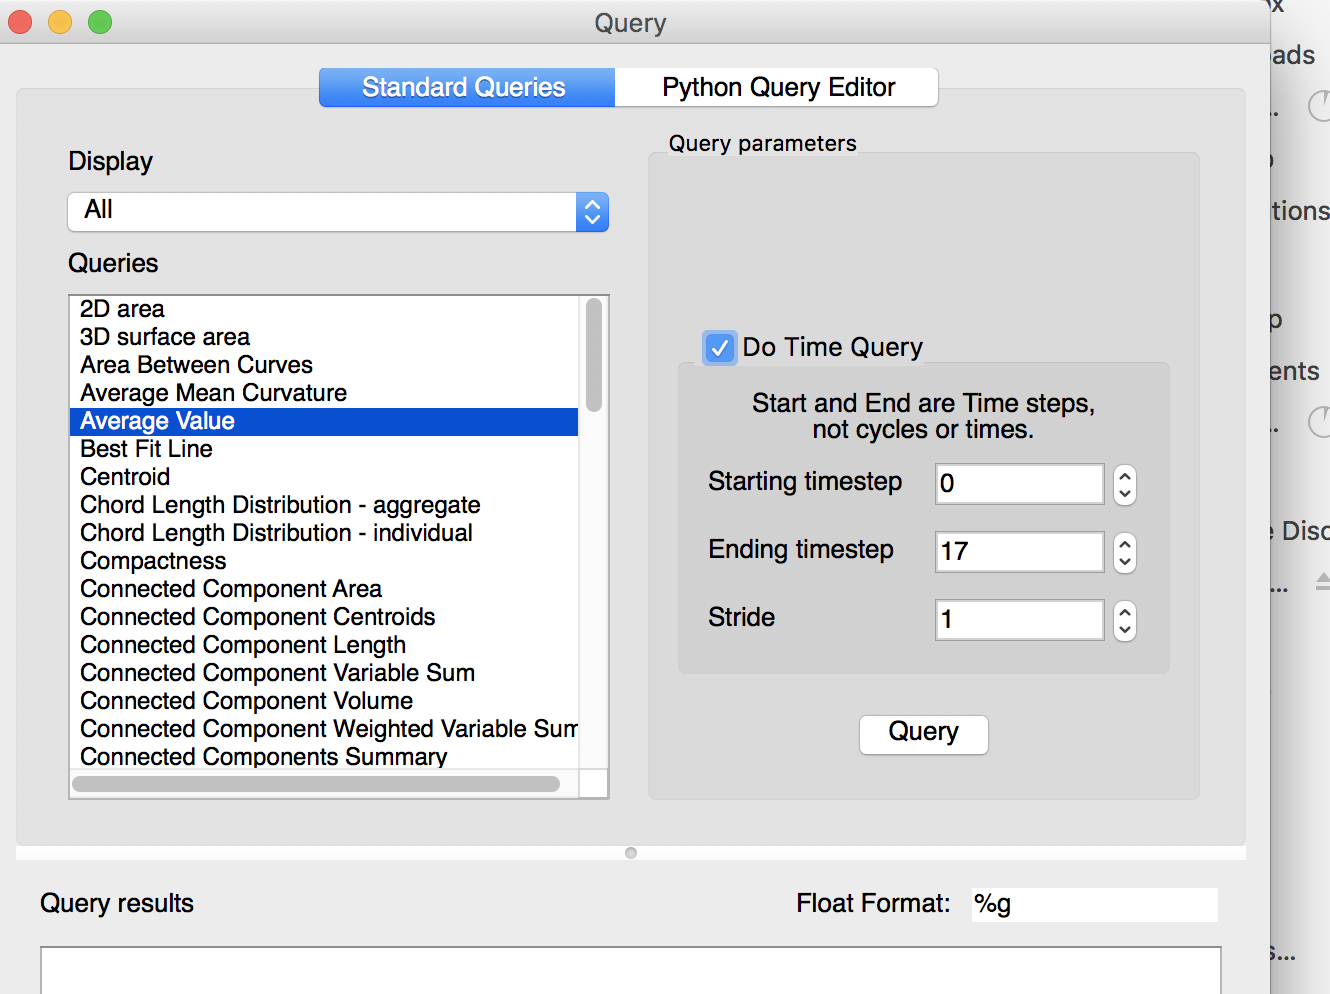
\includegraphics[width=\textwidth]{ch29-2019-query-window.png}
\column{0.58\textwidth}
\footnotesize
``Next, select Query. In this box, there is a list of options on the left that is long \dots\ we'll select `Average Value' \dots\ select the checkbox that says `Do Time Query' \dots\ Hit the `Query' button and wait for a graph.''
\begin{itemize}
  \item The 2019 deck: several queries go onto one graph, another variable (\code{U\_y}, the speed) or another query (Min, Max): ``Each line should show up as a different color'' (not tried in 3.5).
  \item \gui{Average Value} is the area-weighted mean of the cells in the box: on the four frames checked it equals \gui{Weighted Variable Sum} divided by \gui{2D area} to the last digit.
  \item Next slide: the 2019 result and VisIt 3.5's.
\end{itemize}
\end{columns}
\sourcecredit{The 2019 deck, slides 12--13 (VisIt 2.x). The equality: IB/11, VisIt 3.5.0, frames 1, 10, 25, 50.}
\end{frame}

\begin{frame}{The curve, then and now}
\label{fr:avg2}
\begin{columns}[T]
\column{0.48\textwidth}
\centering
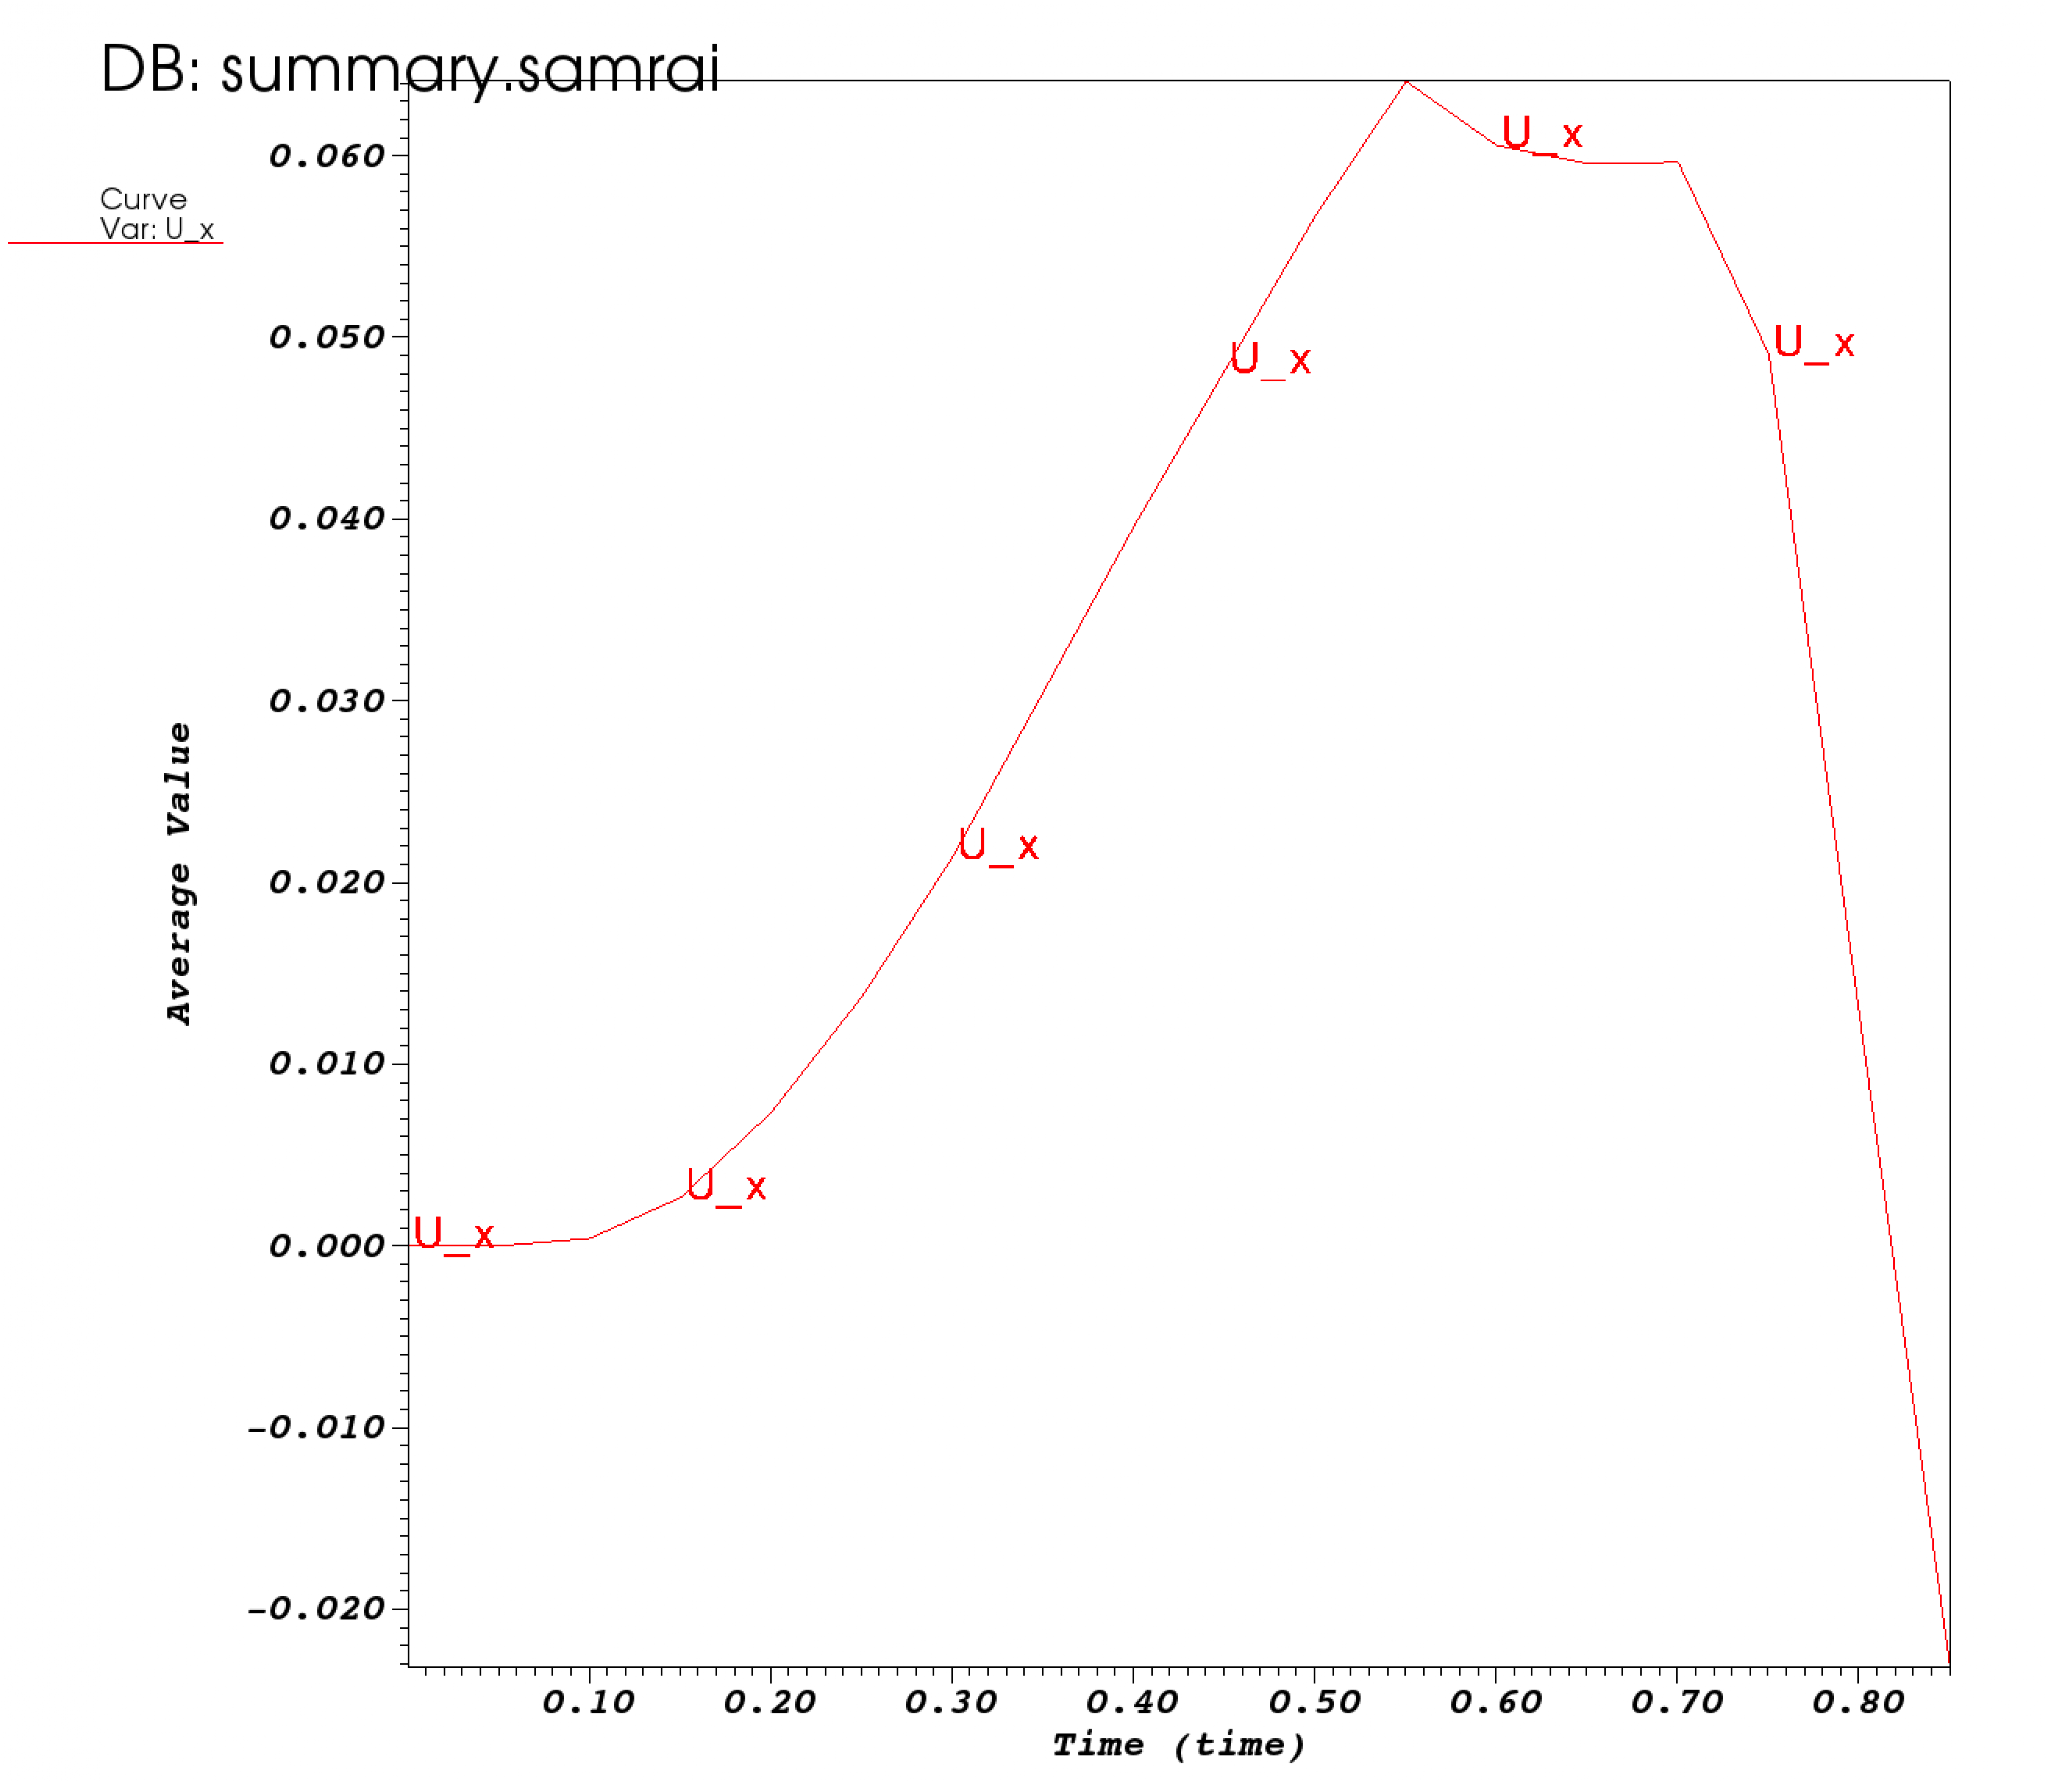
\includegraphics[width=0.92\textwidth]{ch29-2019-average-curve.png}

\scriptsize 2019: the average of \code{U\_x} over the box through the frames of the deck's sample data (``For the limited data set I provided, your graph will look like this'').
\column{0.48\textwidth}
\centering
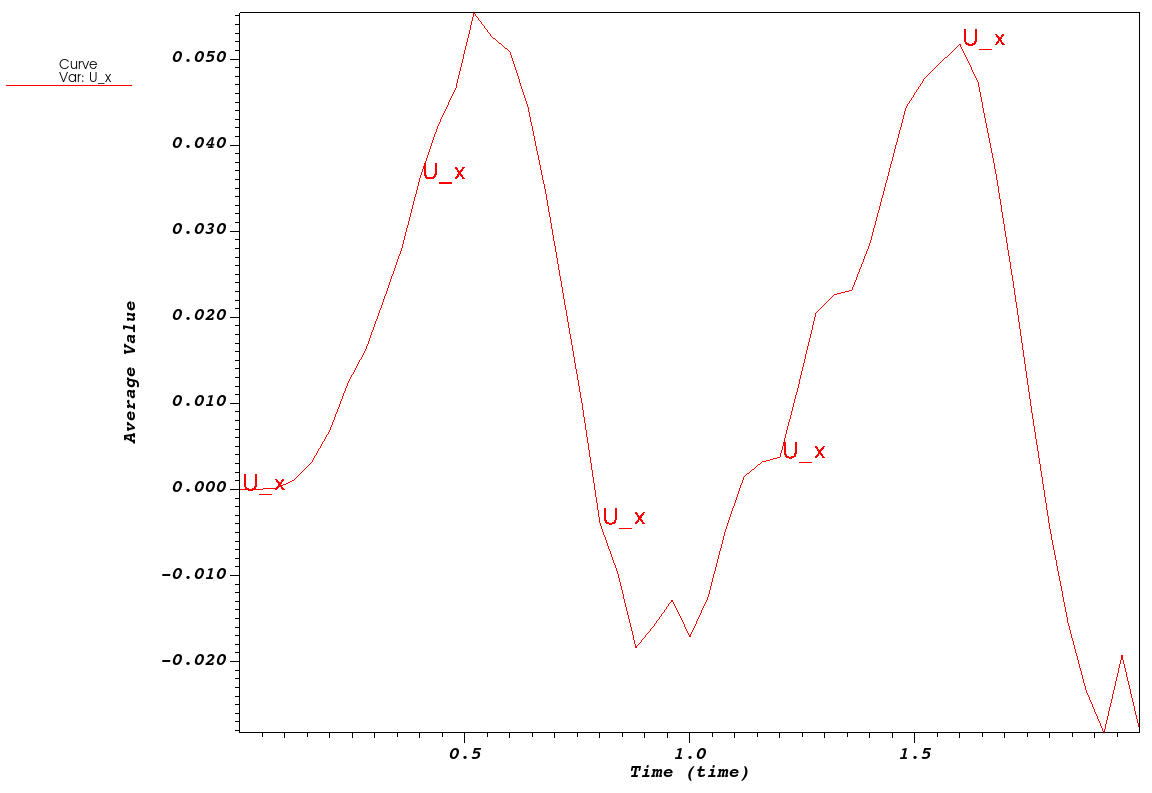
\includegraphics[width=0.92\textwidth]{ch29-average-over-time.png}

\scriptsize VisIt 3.5.0: the same query through time on IB/11 \code{TARGET\_VP}, 51 frames, time on the $x$-axis: two pumping periods. The next slides check it.
\end{columns}
\sourcecredit{Left: the 2019 deck, slide 15. Right: \code{visit\_queries.py}.}
\end{frame}

% 11
\begin{frame}{One average, four ways}
\label{fr:compare}
\centering
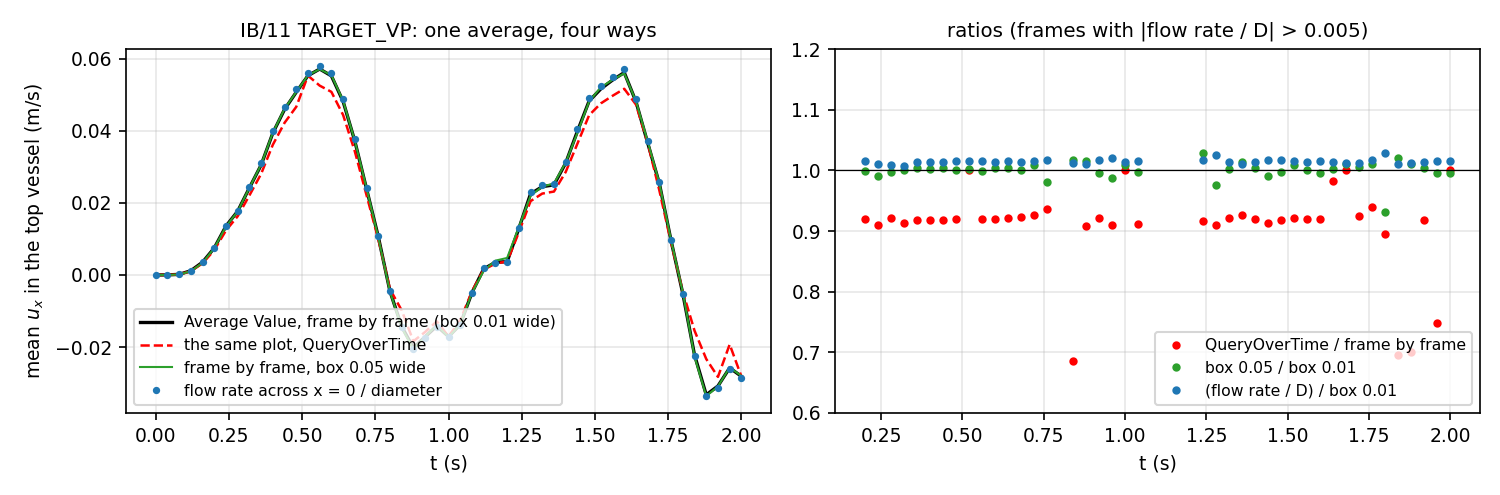
\includegraphics[width=0.95\textwidth]{ch29-average-compare.png}

\scriptsize\raggedright
Left: the box average of \code{U\_x} on IB/11 \code{TARGET\_VP}, frame by frame (black), through time on the same plot (red dashes), frame by frame in a box 5 times wider (green), and the flow rate across the box's line divided by the diameter (blue dots). Right: the ratios, on the frames where the mean speed exceeds 5 mm/s.
\sourcecredit{\code{visit\_queries.py} (VisIt 3.5.0) and \code{tools/ch29\_figures.py}.}
\end{frame}

% 12
\begin{frame}{What the comparison says}
\label{fr:compare2}
\footnotesize
\begin{itemize}
  \item \al{The time query is low.} On the boxed plot, \gui{Query over time} gave 0.919 of the frame-by-frame value (median over the frames with a mean speed above 5 mm/s; 0.69--0.75 on four frames of reversed flow, $t = 0.84$, 1.84, 1.88 and 1.96; exactly 1 at $t = 0.52$, 1.0, 1.68 and 2.0 in this run, but 0.91 and 0.92 at $t = 1.0$ and 2.0 in another session's time query). The same comparison without the Box gave a ratio of 1.0000 on all four frames compared: the trouble is the Box in a time query on this AMR data, in VisIt 3.5.0. With \gui{All} instead of \gui{Some} the time query skipped four frames altogether.
  \item \al{The frame-by-frame value is right.} It agrees with the flow rate across the box's left edge divided by the diameter to within 2.9\,\% on every frame with a mean speed above 5 mm/s (the flow along the straight top vessel is nearly the same at $x = 0$ and $x = 0.01$; the median is 1.5\,\% above the box average, because the \gui{Some} box spans 0.1016 m, a little beyond the walls, where the flow is zero); the time query is 8\,\% off.
  \item \al{The box width matters a little.} A box 5 times wider ($0 \le x \le 0.05$) changed the average by up to 6.9\,\% on the frames with a mean speed above 5 mm/s (by at most 0.001 m/s on any frame): hence the 2019 rule, the same box for every step and every run, and its coordinates in the protocol.
\end{itemize}
\begin{punchbox}
\small Check a time query against the same query on a few single frames (move the time slider, \gui{Query}, compare). If they differ, loop over the frames yourself: \code{visit\_queries.py} does.
\end{punchbox}
\sourcecredit{IB/11 \code{TARGET\_VP}, 51 frames; VisIt 3.5.0 without a window (the GUI was not tried); \code{wsl/final/visit\_ch29\_avg*.sh}.}
\end{frame}

% 13
\begin{frame}{A pick through time at a point}
\label{fr:pick}
\begin{columns}[T]
\column{0.5\textwidth}
\scriptsize
The 2019 recipe: ``Be sure that `Time' is selected \dots\ Open the Query Window. Under `Display' menu, select `Variable-related.' Then, under Queries, select `Pick.' Set your variable \dots\ Enter in your coordinates for single point \dots\ Let's set ours to 0 0.15 0. Select `Pick using coordinate to determine zone' \dots\ `Preserve Picked Coordinate' \dots\ `Create Single Y-Axis plot.' Check the box labeled `Do Time Query' \dots\ Hit Query.''
\begin{itemize}
  \item ``If you use the drop-down box, be sure to manually erase the previous variable (or the word `default') because selecting a new variable will not erase the last one used.''
  \item \al{Zone or node.} The 2019 deck picks by zone, as Waldrop's 2015 original (for IBAMR) did; the IB2d version of her guide changed it to ``coordinate to determine node''. In VisIt 3.5 a zone pick through time on \code{U\_x}, which is node-centred in IBAMR 0.19's output, refuses: ``The centering of the pick-through-time (zone) does not match the centering of the plot's current variable (node). Please try again with the appropriately centered Pick'' (VisIt's words). Use the node pick.
\end{itemize}
\column{0.48\textwidth}
\centering
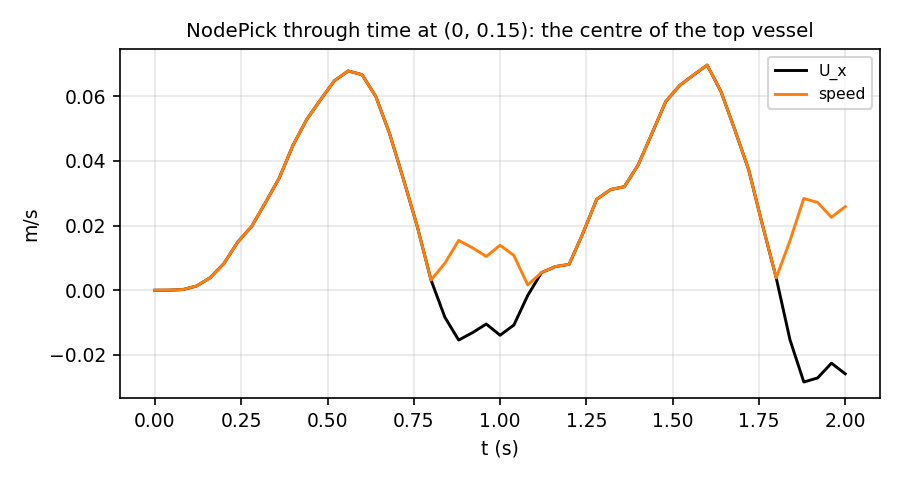
\includegraphics[width=\textwidth]{ch29-pick.png}

\scriptsize\raggedright
A node pick through time at $(0, 0.15)$ of \code{U\_x} and the speed, on one $y$-axis: $u_x$ peaks at 0.070 m/s ($t = 1.6$) and reverses to $-0.028$ ($t = 1.88$); where it is negative the speed is its absolute value.
\end{columns}
\sourcecredit{The 2019 deck, slides 16--18; Waldrop's guide. IB/11 \code{TARGET\_VP}, VisIt 3.5.0 (\code{NodePick(coord=..., do\_time=1, preserve\_coord=1, curve\_plot\_type=0)}).}
\end{frame}

% 14
\begin{frame}{A lineout: a variable along a line at one time}
\label{fr:lineout}
\begin{columns}[T]
\column{0.42\textwidth}
\centering
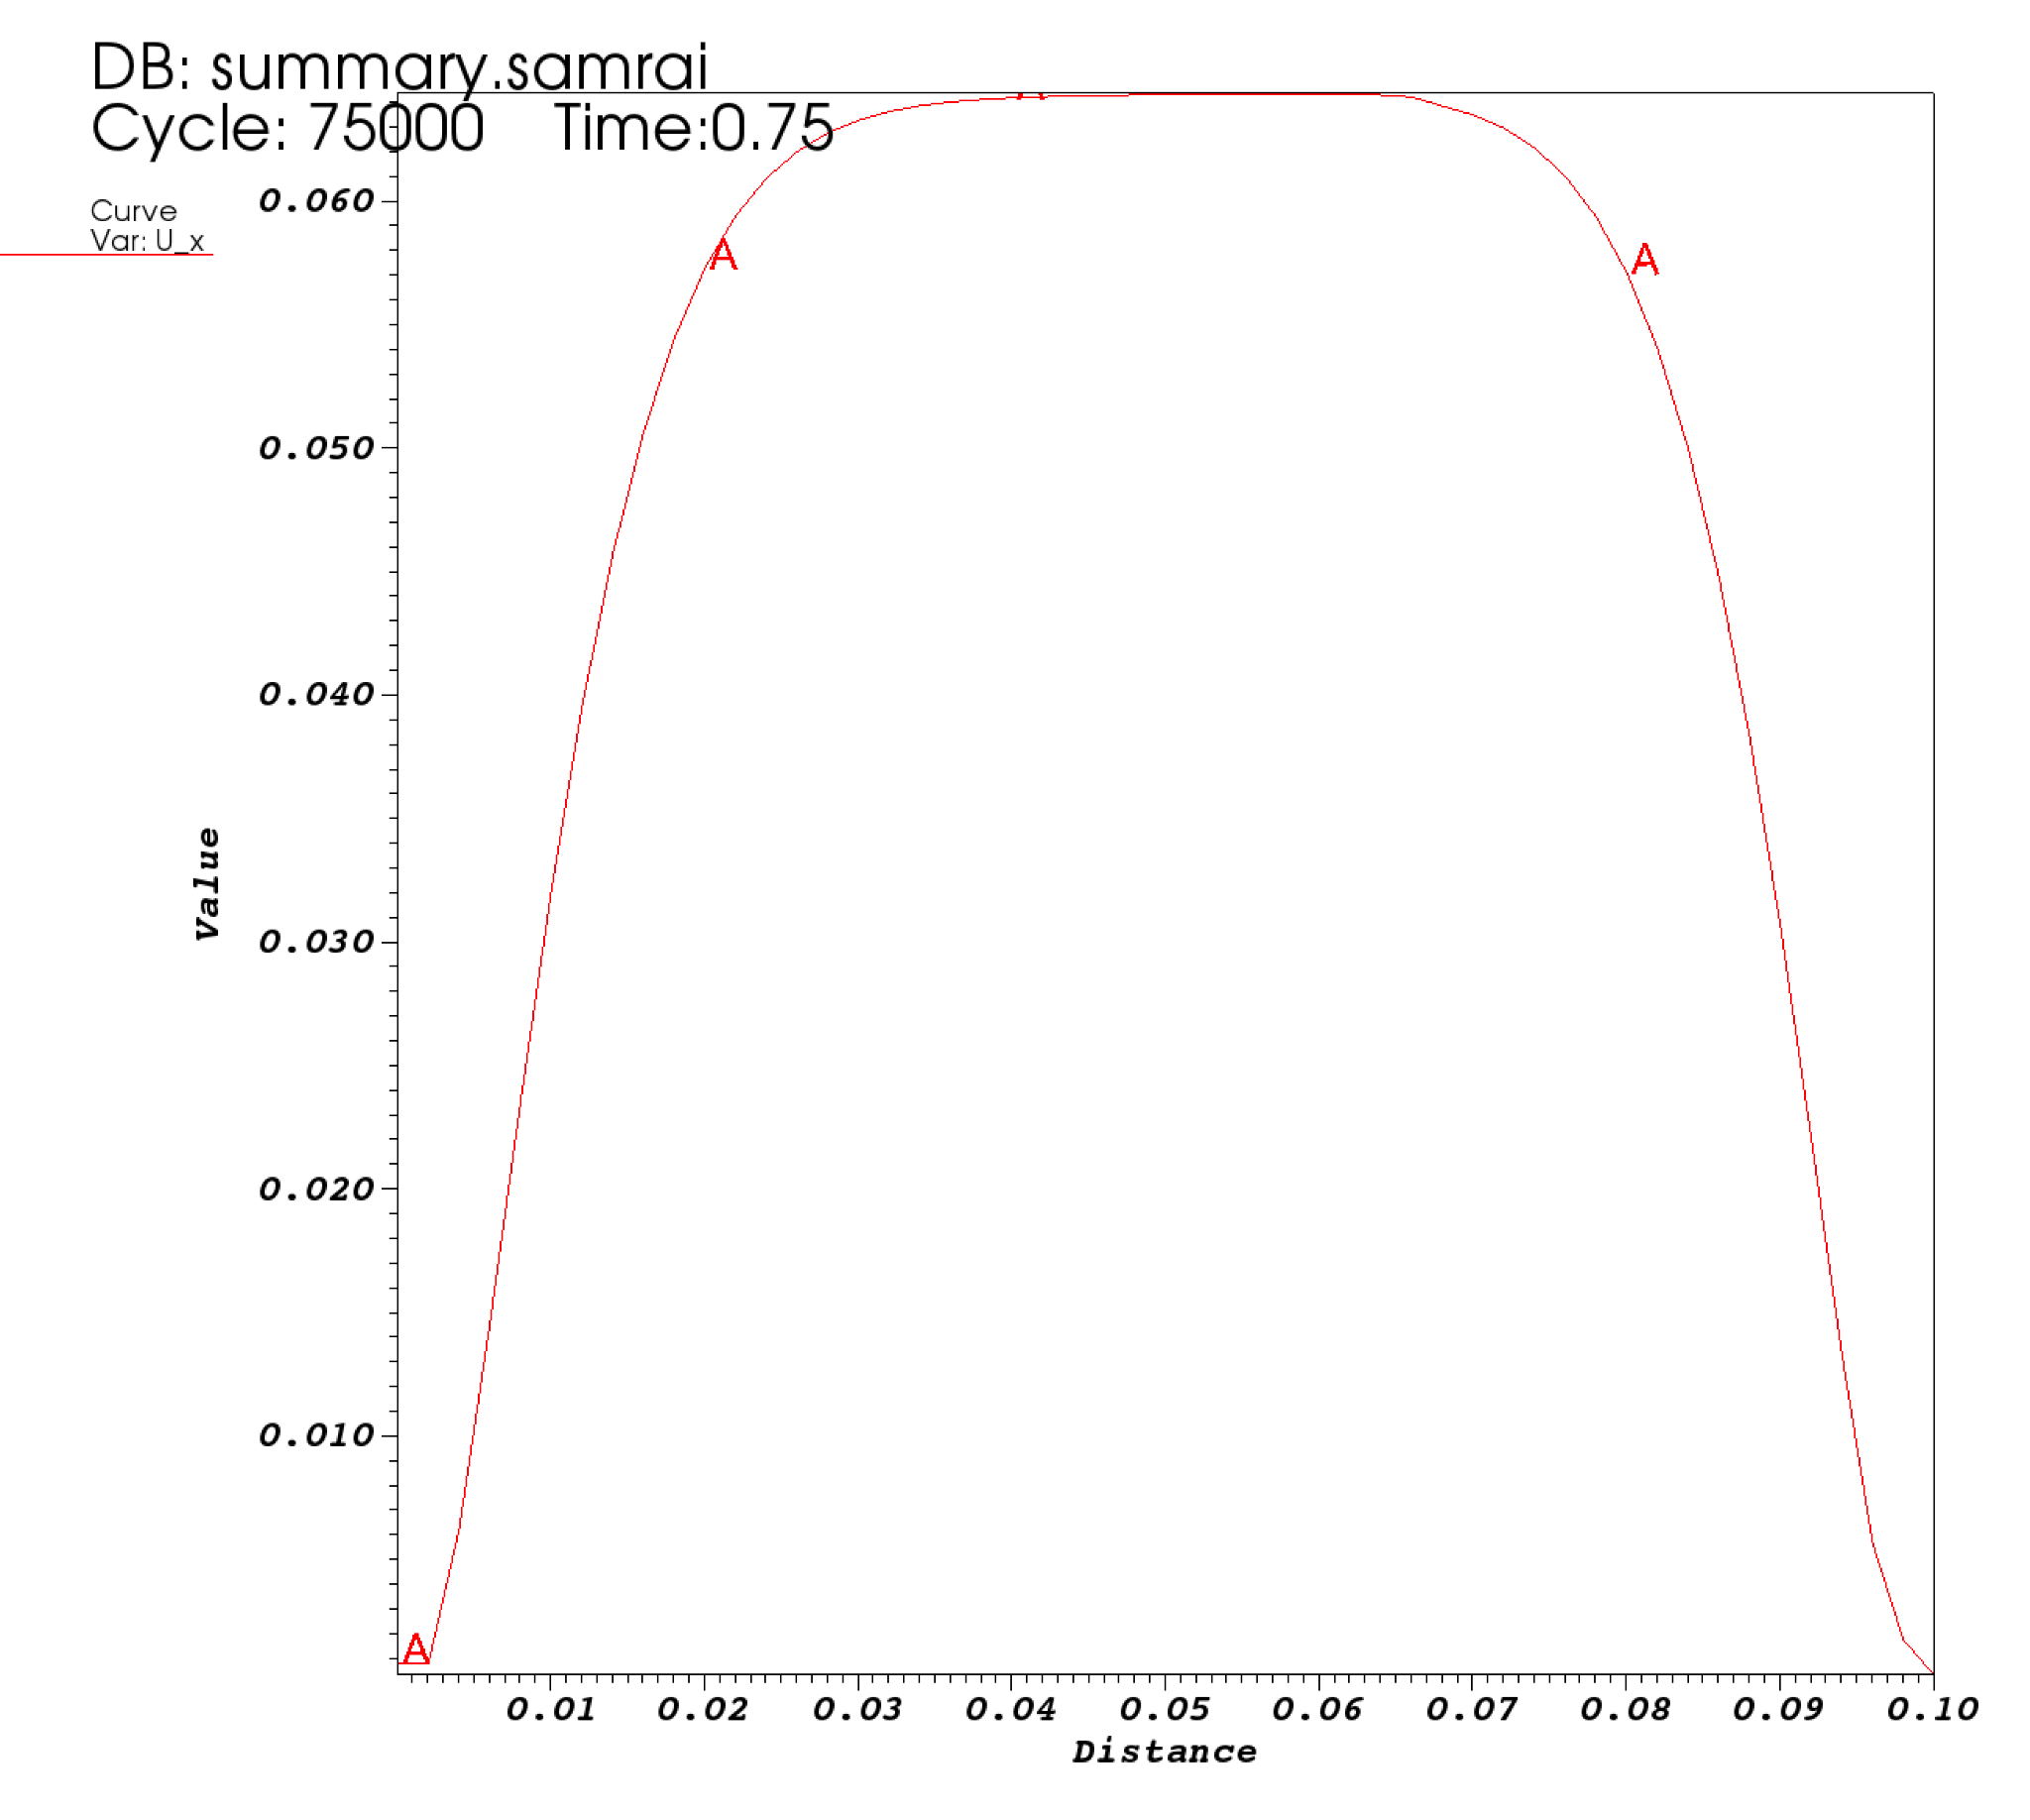
\includegraphics[width=0.95\textwidth]{ch29-2019-lineout-curve.png}

\scriptsize The 2019 lineout across the vessel (VisIt 2.x, $t = 0.75$): a flat core and steep walls.
\column{0.56\textwidth}
\footnotesize
``If you want to analyze data along a line in your plot area \dots\ under Queries, select `Lineout.' \dots\ Enter in your coordinates for the beginning and end of the line \dots\ Let's set ours to 0 0.1 0 and 0 0.2 0. Click Use Sampling. The default number of 50 is typically pretty good. Hit Query.''
\begin{itemize}
  \item A lineout is one frame. For a lineout in every frame, loop over the frames (slide \ref{fr:script}).
\end{itemize}
\end{columns}
\sourcecredit{The 2019 deck, slides 19--21.}
\end{frame}

\begin{frame}{The lineout in VisIt 3.5, and sampling}
\label{fr:lineout2}
\begin{columns}[T]
\column{0.5\textwidth}
\centering
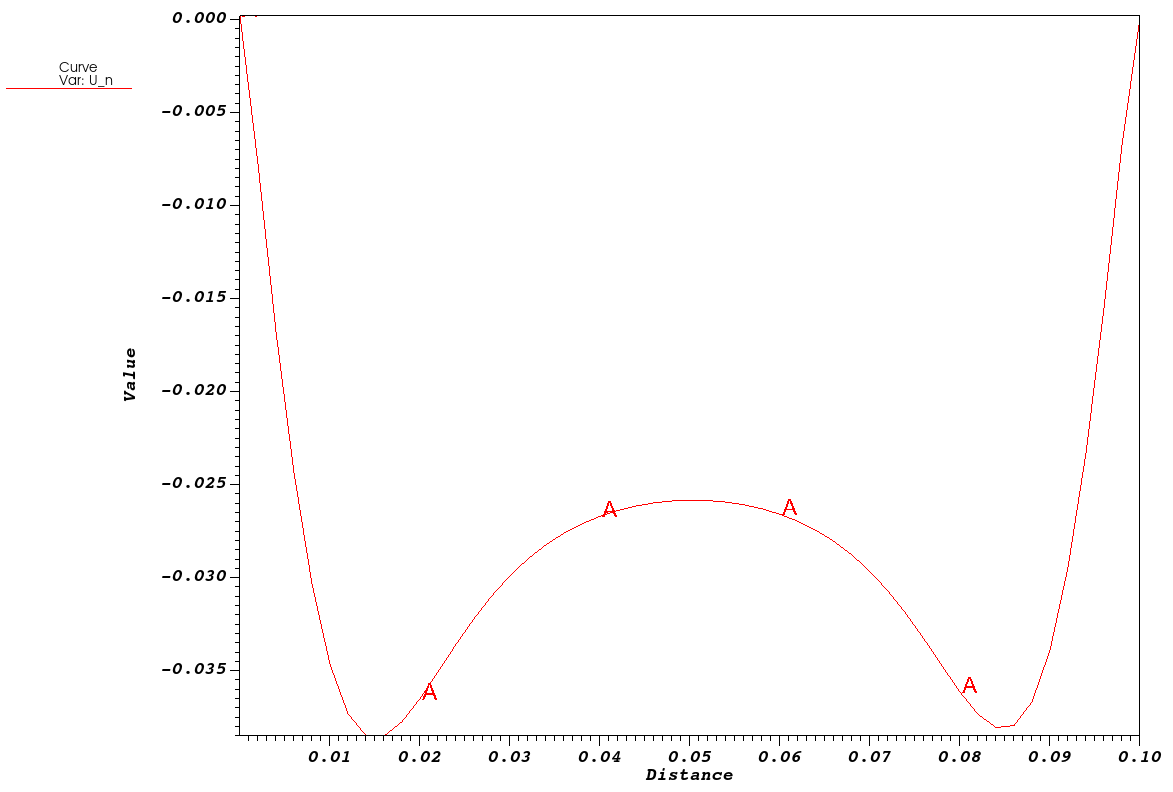
\includegraphics[width=0.95\textwidth]{ch29-lineout.png}
\column{0.48\textwidth}
\footnotesize
\begin{itemize}
  \item The same line on \code{TARGET\_VP} at $t = 2$ in VisIt 3.5 (the variable is \code{U\_n}, the velocity across the line, slide \ref{fr:flux}: here \code{U\_x}), while the flow reverses: the fluid near the walls moves backwards faster than the core (slide \ref{fr:profiles}).
  \item With sampling, 50 samples give 51 points, equally spaced. Without it, VisIt takes the value wherever the line crosses a cell: 52 points here ($0.1/\Delta x = 51.2$ cells); on a coarse level, few.
\end{itemize}
\end{columns}
\sourcecredit{IB/11 \code{TARGET\_VP}, VisIt 3.5.0 (\code{Lineout(..., use\_sampling=1, num\_samples=50)}).}
\end{frame}

% 15
\begin{frame}{The profile across the vessel through a pumping period}
\label{fr:profiles}
\begin{columns}[T]
\column{0.55\textwidth}
\centering
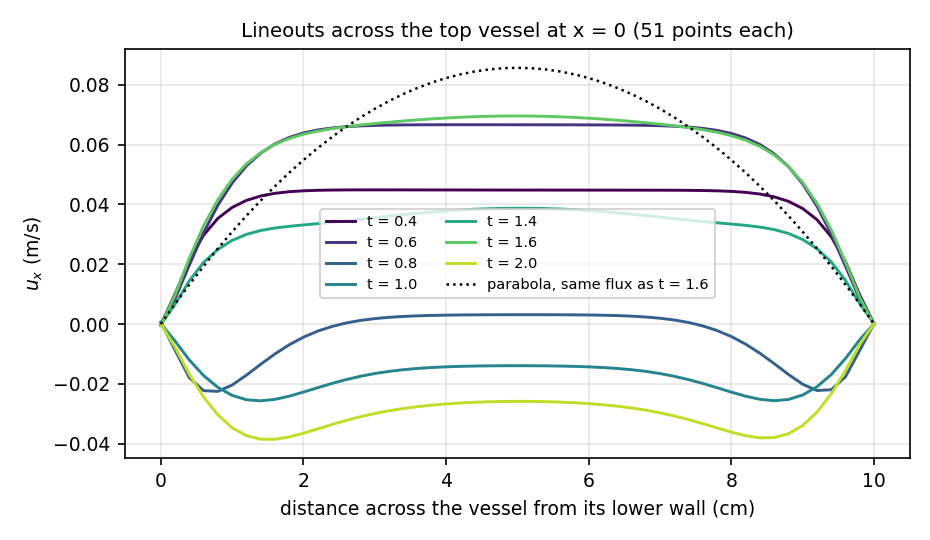
\includegraphics[width=\textwidth]{ch29-profiles.png}
\column{0.43\textwidth}
\footnotesize
\begin{itemize}
  \item Lineouts across the top vessel at $x = 0$, one in every frame (50 samples, 51 points each): seven of them shown.
  \item Not parabolas. At $t = 1.6$ the profile is a flat plug with a centre speed of 0.070; a parabola with the same flow rate would peak at 0.086 (dots).
  \item When the flow reverses ($t = 0.8$, $2.0$), the fluid near the walls turns first: at $t = 2.0$ the profile's extreme, $-0.0385$, lies 16 mm from the wall, and the centre has only $-0.026$.
  \item Both are oscillatory flow at a Womersley number of 10 (chapter 8b): viscosity reaches only a thin layer at the wall in one period, and the core moves as a plug.
\end{itemize}
\end{columns}
\sourcecredit{IB/11 \code{TARGET\_VP}; \code{visit\_queries.py} (\code{lineouts.csv}), \code{tools/ch29\_figures.py}.}
\end{frame}

% 16
\begin{frame}{From a lineout to a flow rate}
\label{fr:flux}
\footnotesize
\begin{itemize}
  \item The flow rate per unit depth across a line is $Q = \int \mathbf{u}\cdot\mathbf{n}\,ds$. On the vertical line $(0, 0.1)$--$(0, 0.2)$, $\mathbf{u}\cdot\mathbf{n} = u_x$.
  \item For any line, define the velocity across it: with the line from $(x_0, y_0)$ to $(x_1, y_1)$, length $L$, the normal to its right is $\mathbf{n} = (y_1 - y_0,\ -(x_1 - x_0))/L$, and \code{U\_n = n\_x*U[0] + n\_y*U[1]} with the numbers put in (\gui{Controls $\to$ Expressions}).
  \item Lineout of \code{U\_n} with sampling, then \gui{Query $\to$ Integrate} on the curve in window 2: the area under it. At $t = 2$ on \code{TARGET\_VP}: $-0.0028609$ m$^2$/s, the same as the trapezoid rule on the 51 points.
  \item Through time: one lineout per frame, integrated (\code{visit\_queries.py} writes \code{averages.csv} with \code{flow\_rate\_line} for every frame).
\end{itemize}
\begin{punchbox}
\small A box average and a flow rate answer the same question in a straight vessel; on a moving or curved part they do not, and a line is easier to place.
\end{punchbox}
\sourcecredit{IB/11 \code{TARGET\_VP}, VisIt 3.5.0.}
\end{frame}

% 17
\begin{frame}{The flow round the loop, on six lines}
\label{fr:loop}
\centering
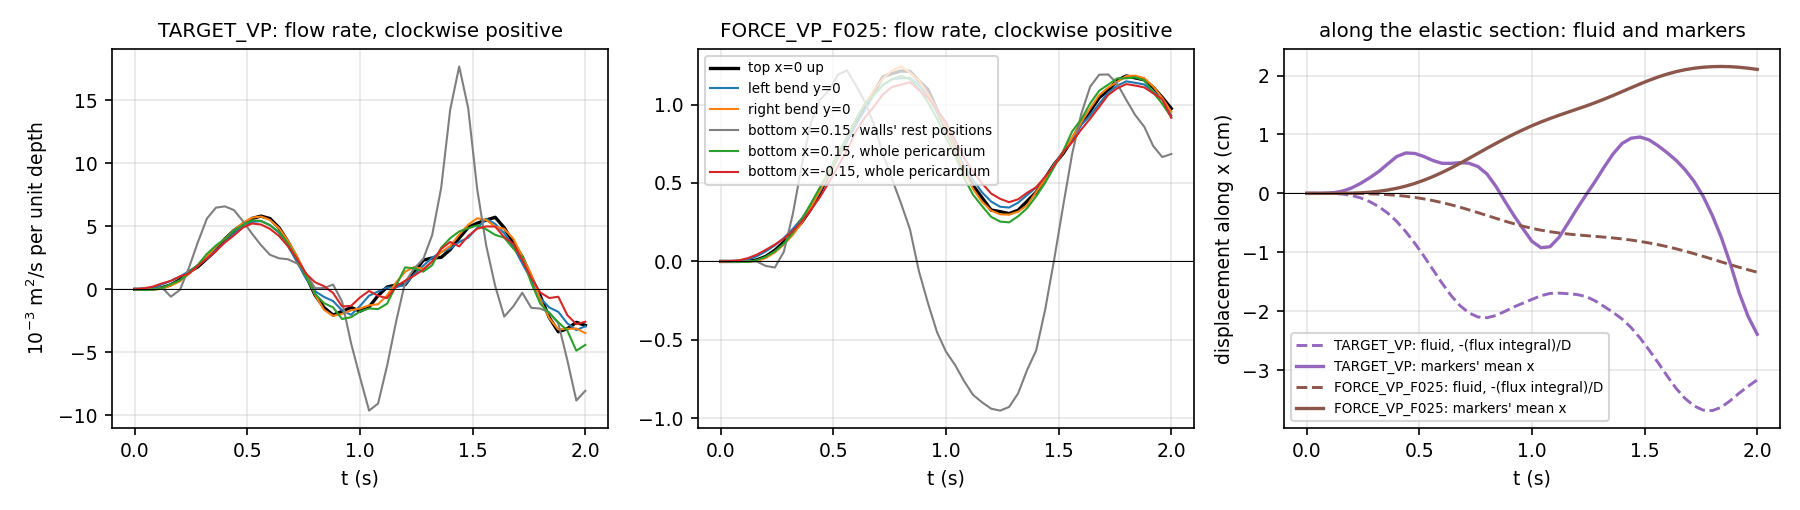
\includegraphics[width=\textwidth]{ch29-loopflux.png}

\scriptsize\raggedright
Left and middle: the flow rate on the six lines of slide \ref{fr:map}, clockwise positive, for the two suction modes of IB/11. Right: along the elastic section, how far the fluid moved (minus the time integral of the top line's flow rate, divided by $D$; dashed) and how far the markers' mean $x$ moved (solid).
\sourcecredit{\code{visit\_queries.py} on six lines per run (\code{wsl/final/ch29\_loopflux*.sh}); the markers' mean $x$ from \code{lag\_data.visit} (\gui{Variable Sum} of their $x$ over 121 points).}
\end{frame}

% 18
\begin{frame}{What the six lines say}
\label{fr:loop2}
\scriptsize
\begin{center}
\begin{tabular}{@{}lrr@{}}
\toprule
line (mean over 0--2 s, m$^2$/s per unit depth) & \code{TARGET\_VP} & \code{FORCE\_VP} \\
\midrule
top straight, $x = 0$ & $1.582 \times 10^{-3}$ & $6.688 \times 10^{-4}$ \\
left bend, $y = 0$ & $1.578 \times 10^{-3}$ & $6.675 \times 10^{-4}$ \\
right bend, $y = 0$ & $1.578 \times 10^{-3}$ & $6.687 \times 10^{-4}$ \\
elastic section, $x = \pm 0.15$, whole pericardium & $1.42$, $1.69 \times 10^{-3}$ & $6.55$, $6.60 \times 10^{-4}$ \\
elastic section, $x = 0.15$, walls' rest positions & $1.20 \times 10^{-3}$ & $2.51 \times 10^{-4}$ \\
\bottomrule
\end{tabular}
\end{center}
\footnotesize
\begin{itemize}
  \item The fluid is incompressible, so the flow round a closed loop is one number: the top and both bends agree to 0.3\,\%. Both suction modes turn the loop clockwise, $-x$ along the elastic section. \code{TARGET\_VP} reverses within each period; \code{FORCE\_VP} never does.
  \item Across the elastic section only a line over the whole pericardium comes within 10\,\% (its two lines give 1.42 and $1.69 \times 10^{-3}$, and 6.55 and $6.60 \times 10^{-4}$); a line between the walls' rest positions misses the moving tube.
  \item \al{The markers are not the flow.} The \code{FORCE\_VP} markers drift $+2.1$ cm in two periods while the fluid along the elastic section moves $-1.3$ cm (slide \ref{fr:loop}); 22 of the 121 markers start on the walls' rest positions and ride with the walls. Chapter 9b read the markers as the flow; it is corrected.
\end{itemize}
\sourcecredit{The numbers: \code{tools/ch29\_figures.py} on the six \code{flux\_*.csv} files of each run.}
\end{frame}

% 19
\begin{frame}{The same flow rate from a reader of your own}
\label{fr:cross}
\footnotesize
\begin{itemize}
  \item Chapter 33 computed the flow rate of \code{FORCE\_VP} across the top straight at $x = \pm 0.15$ with its own reader of the SAMRAI files (\code{examples/analysis/flow\_rate.py}): means $6.64$ and $6.65 \times 10^{-4}$ m$^2$/s.
  \item VisIt's lineouts on the line at $x = 0.15$, $y \in [0.1, 0.2]$, integrated frame by frame: a mean of $6.656 \times 10^{-4}$ over the 51 frames ($6.69 \times 10^{-4}$ as a time integral). Two independent routes agree to 0.1\,\% (with chapter 33's $6.65$, given for $x = 0.15$; both plain means over the frames).
  \item That is the habit this chapter asks for: every number from two routes that share nothing but the data.
\end{itemize}
\begin{punchbox}
\small A number measured once is a guess with a decimal point. A number measured two ways that agree is a result; two ways that disagree are a finding (slides \ref{fr:compare2} and \ref{fr:loop2}).
\end{punchbox}
\sourcecredit{Chapter 33, slide ``The flow rate of the valveless pump''; \code{visit\_queries.py} with \code{line=0.15,0.10,0.15,0.20}.}
\end{frame}

% 20
\begin{frame}[fragile]{Exporting curves}
\label{fr:export}
\begin{columns}[T]
\column{0.52\textwidth}
\scriptsize
``At the top of the main window, select Active Window: 2 or whichever window your plot is in. Highlight the curve \dots\ under `File,' select `Set Save Options\dots' \dots\ select the file type `curve.' \dots\ Change the file name and output directory. Click `Save.'''
\begin{itemize}
  \item ``VisIt outputs data as a two-column text file with a short header, delineated by spaces (instead of commas, like a csv file).''
  \item VisIt 3.5 writes a line \code{\# name} before each curve, then one \code{x y} pair per line; a pick of two variables through time gives two curves in one file. In a script, \code{SaveWindow} with \code{format = CURVE} on the curve window (it kept the name and folder given, unlike the VTK export of chapter 33).
\end{itemize}
\column{0.46\textwidth}
\begin{lstlisting}[style=tiny]
# U_x
0 0
0.03999999910593033 2.368893728998955e-05
0.07999999821186066 0.0001810442772693932
...
# speed
0 0
0.03999999910593033 3.270131855970249e-05
...
\end{lstlisting}
\scriptsize The pick through time of slide \ref{fr:pick} as VisIt wrote it (shortened).
\end{columns}
\sourcecredit{The 2019 deck, slides 22--23; Waldrop's guide. VisIt 3.5.0.}
\end{frame}

% 21
\begin{frame}[fragile]{Reading curves: Python, MATLAB, R}
\label{fr:read}
\begin{columns}[T]
\column{0.5\textwidth}
\begin{lstlisting}[style=pytiny]
# Python: examples/analysis/read_curve.py
from read_curve import read_curve
c = read_curve("pick.curve")   # {'U_x': (t, u), 'speed': (t, s)}
t, u = c["U_x"]
# one curve per file: numpy.loadtxt(path, comments="#")
\end{lstlisting}
\begin{lstlisting}[style=tiny]
% MATLAB or Octave: examples/analysis/read_curve.m
c = read_curve('pick.curve');   % c(k).name, c(k).x, c(k).y
plot(c(1).x, c(1).y)
% one curve per file (the 2018 lecture):
d = importdata('average.curve');  t = d.data(:,1);
\end{lstlisting}
\begin{lstlisting}[style=tiny]
# R (Waldrop's guide)
data <- read.table("visit10000.curve", header=FALSE, sep="")
\end{lstlisting}
\column{0.48\textwidth}
\footnotesize
\begin{itemize}
  \item The 2018 lecture's \code{importdata}: ``time is the first column \dots\ velocity is the second''; Octave 8.4 returned a struct whose \code{data} is $51 \times 2$ for the average's file.
  \item For a file with two curves (the pick), \code{importdata} and \code{loadtxt} run them together (Octave 8.4's \code{importdata}: $103 \times 2$, an \code{NA} row where the second name was; \code{loadtxt}: $102 \times 2$); \code{read\_curve} keeps them apart. Both readers were run on this chapter's files.
  \item Waldrop's R line gives two columns \code{data\$V1} (time) and \code{data\$V2} (the variable); its \code{sep=""} means any white space. R was not run here.
\end{itemize}
\end{columns}
\sourcecredit{The 2018 lecture ``3B -- Analyzing your IBFE simulation'', slide 16; Waldrop's guide.}
\end{frame}

% 22
\begin{frame}{The IBFE version: a box above the corals (2018)}
\label{fr:ibfe}
\footnotesize
``Graphing spatially averaged vertical flow. Make a pseudocolor plot of \code{U\_y}. Use \gui{Operators $\to$ Selection $\to$ Box} to average in a box. Draw a box above the corals of whatever size you like. You must specify range in x, y and z. What you pick does not matter too much as long as it's consistent.''
\begin{itemize}
  \item Then the same time query (\gui{Query over time options}: time; \gui{Average Value}, \gui{Do Time Query}) and the curve saved for MATLAB.
  \item The 2018 deck did it on a cluster whose VisIt could not read \code{.ex2} files, so the coral meshes went through VTK (chapter 28); the fluid's box average needs only \code{dumps.visit}.
  \item ``What you pick does not matter too much as long as it's consistent'': true for comparing runs, but a box 5 times wider changed the IB/11 average by up to 7\,\% (on frames with a mean speed above 5 mm/s); report the box with the number.
  \item In 3D the box is a volume, \gui{Average Value} its volume-weighted mean, and the time query deserves the same check as in 2D (slide \ref{fr:compare2}).
\end{itemize}
\sourcecredit{The 2018 lecture ``3B -- Analyzing your IBFE simulation'', slides 12--16 (VisIt 2.12).}
\end{frame}

% 23
\begin{frame}{Expressions for analysis}
\label{fr:expr}
\footnotesize
\begin{center}
\begin{tabular}{@{}L{0.16\textwidth}L{0.3\textwidth}L{0.48\textwidth}@{}}
\toprule
name & definition & what for \\
\midrule
\code{U\_x}, \code{U\_y} & \code{U[0]}, \code{U[1]} & components (IBAMR 0.19 writes the vector only) \\
\code{speed} & \code{magnitude(U)} & instead of VisIt's \code{U\_magnitude} beside a plot from a second database \\
\code{U\_n} & \code{nx*U[0] + ny*U[1]}, the line's numbers in & the velocity across a line, for a flow rate \\
\code{vortmag} & \code{magnitude(Omega)} & 3D vorticity magnitude (chapter 27) \\
\code{dX} & \code{\{dX\_0, dX\_1, dX\_2\}} & an IBFE body's displacement in 3D (VisIt builds the 2D one itself; chapter 28) \\
\bottomrule
\end{tabular}
\end{center}
\begin{itemize}
  \item An expression is computed when a plot or query asks for it, frame by frame, and saved in the session, not in the data (chapter 26).
  \item VisIt's expression language has the usual functions (\code{abs}, \code{sqrt}, \code{min}, \code{max}, \code{if}), vector operations (\code{dot}, \code{cross}, \code{curl}, \code{gradient}) and coordinates (\code{coord(mesh)}): the markers' mean $x$ of slide \ref{fr:loop} was \code{coord(markers\_512\_vertices)[0]}, summed with \gui{Variable Sum} and divided by 121.
\end{itemize}
\sourcecredit{VisIt 3.5.0; this chapter's and chapters 26--28's expressions.}
\end{frame}

% 24
\begin{frame}[fragile]{All of it, scripted}
\label{fr:script}
\begin{columns}[T]
\column{0.52\textwidth}
\begin{lstlisting}[style=shell]
visit -nowin -cli -s visit_queries.py -- \
      viz_IB2d/dumps.visit out \
      box=0,0.01,0.10,0.20 point=0,0.15 \
      line=0,0.10,0,0.20 samples=50
\end{lstlisting}
\scriptsize \code{examples/analysis/visit\_queries.py} runs inside VisIt's Python without a window (about 30 s for IB/11's 51 frames) and writes:
\begin{itemize}
  \item \code{ch29-box.png}; the curve windows as PNG and \code{.curve}: the average through time, the pick through time, the lineout (sampled; the unsampled one as \code{.curve} only);
  \item \code{averages.csv}: per frame, the box average (frame by frame) and the flow rate across the line;
  \item \code{lineouts.csv}: every frame's lineout.
\end{itemize}
\column{0.46\textwidth}
\begin{lstlisting}[style=pytiny]
for k in range(N):                       # every frame
    SetTimeSliderState(k)
    Query("Average Value")               # on the boxed plot
    avg = GetQueryOutputValue()
    Lineout(start_point=(0, 0.1, 0), end_point=(0, 0.2, 0),
            vars=("U_n",), use_sampling=1, num_samples=50)
    SetActiveWindow(2)                   # the lineout's window
    xy = GetPlotInformation()["Curve"]   # x0, y0, x1, y1, ...
    DeleteAllPlots(); SetActiveWindow(1)
\end{lstlisting}
\scriptsize The loop that replaces the time query (simplified: the script runs two loops, and makes the lineouts on a plot of \code{U\_x} without the Box). Chapter 32 is about VisIt's Python; chapter 31 runs it on the cluster.
\end{columns}
\end{frame}

% 25
\begin{frame}{When the analysis goes wrong}
\label{fr:trouble}
\scriptsize
\begin{tabular}{@{}L{0.42\textwidth}L{0.53\textwidth}@{}}
\toprule
what you see & what to do \\
\midrule
the box changes every plot, or the structure disappears & untick ``Apply operators to all plots'' (and ``\dots subset selections \dots'') before adding the Box \\
\code{U\_x} is not in the menu & IBAMR 0.19 writes \code{U} only: define \code{U\_x = U[0]} \\
the time axis shows cycles & \gui{Query over time options}: \gui{Time} \\
a time query disagrees with single frames & check a few frames by hand; loop over frames (slide \ref{fr:compare2}) \\
a time query skips frames & seen with the Box set to \gui{All}: use \gui{Some}, or loop over the frames \\
a scripted time query on the boxed plot gives no curve (``The Curve plot of variable U\_x yielded no data'') & it had \code{use\_actual\_data=0}: use \code{1} \\
``The centering of the pick-through-time (zone) does not match \dots'' & pick by node \\
the pick follows the old variable & erase the previous variable (or ``default'') in the box \\
a lineout has few, uneven points & tick \gui{Use sampling} \\
a flow rate has the wrong sign & the line's direction: positive flow crosses it from left to right \\
the flow rate across a moving part is small & the line misses the structure: span the whole region (slide \ref{fr:loop2}) \\
the markers say one thing, the flow rate another & believe the flow rate; markers are a few parcels \\
\code{importdata} runs two curves together & \code{read\_curve} \\
\bottomrule
\end{tabular}
\sourcecredit{The 2019 deck and Waldrop's guide, with what happened while this chapter was made (VisIt 3.5.0).}
\end{frame}

% 26
\begin{frame}{Exercises}
\label{fr:exercises}
\footnotesize
\begin{enumerate}
  \item Fill in \code{templates/analysis\_protocol.md} for one measurement of your own, and ask someone to repeat it from the protocol alone.
  \item Repeat slide \ref{fr:compare} by hand in the GUI: the box, \gui{Average Value} on three frames, then the time query. Do the two agree in the GUI?
  \item Run \code{visit\_queries.py} on \code{FORCE\_VP} with the default box, point and line. How does the pick through time differ from \code{TARGET\_VP}'s?
  \item Measure the flow rate of \code{TARGET\_PERI} (the target wave) on the top straight and on both bends. Which way does it pump, and do its markers agree?
  \item The guide's own example: IB2d's \code{Rubberband\_with\_Springs}, \code{Omega} in the box $0.5 \le x \le 1$, $0 \le y \le 0.5$, its average through time, and a node pick at $(0.75, 0.25)$ (chapter 4a runs it).
  \item Make the lineout of slide \ref{fr:profiles} at the moment of largest flow and fit a parabola to the inner half: how far from Poiseuille is it?
  \item Read one of your \code{.curve} files in R with the guide's \code{read.table} line, and in Python with \code{read\_curve}.
\end{enumerate}
\end{frame}

% 27
\begin{frame}{Summary}
\label{fr:summary}
\footnotesize
\begin{itemize}
  \item Write the analysis down as you go: a protocol with every box, point and line, a data sheet per run, a report (templates in \code{examples/analysis/templates}).
  \item A Box restricts a plot; \gui{Average Value} is the area-weighted mean over its cells (\gui{Some} or \gui{All}: say which).
  \item \gui{Query over time} with \gui{Time} as the axis; on IB/11 with a Box it was 8\,\% low against the same query frame by frame, so check it or loop over the frames.
  \item A node pick through time follows a point; a lineout with sampling samples a line; integrated, it is the flow rate across the line.
  \item The flow round IB/11's loop is one number on every line across its rigid parts (to 0.3\,\%), and close to it on a line across the whole pericardium, clockwise in both suction modes; the markers' drift is not that number.
  \item Curves leave VisIt as \code{.curve} text and come back with \code{read\_curve} (Python, MATLAB/Octave), \code{importdata}, \code{loadtxt} or R's \code{read.table}.
  \item Measure every number two ways.
\end{itemize}
\vspace{1mm}
Next: chapter 30 (movies), 31 (VisIt on the cluster), 32 (VisIt from the command line and Python).
\end{frame}

% 28
\begin{frame}{References and credits}
\label{fr:refs}
\scriptsize
\begin{itemize}
  \item L. Waldrop, ``Data analysis in VisIt'', MATH 769 (16 February 2015; VisIt 2.5.2, IBAMR data); its 2017 version for IB2d's \code{.vtk} output is quoted on slides \ref{fr:practice}, \ref{fr:tips}, \ref{fr:pick}, \ref{fr:export}, \ref{fr:read}.
  \item L.\,A. Miller, ``4 -- Visit Data Analysis -- Sampling and Time Queries'' (2019, adapted from Waldrop's tutorial; pictures reused: slides 11, 13, 15, 21), and ``Lecture 9: Sampling, averaging, and analyzing data in Visit'' (its title slide: ``Lecture 9 -- Visit, Sampling and Time Queries''; adapted from Waldrop's and N. Battista's tutorials); ``3B -- Analyzing your IBFE simulation'' (2018), slides 12--16.
  \item VisIt: H. Childs et al., ``VisIt: An end-user tool for visualizing and analyzing very large data'', in \emph{High Performance Visualization}, CRC Press (2012) 357--372; version 3.5.0 (Linux), run without a window.
  \item The runs: \code{examples/IB/11-heart-tube-pump} (\code{TARGET\_VP}, \code{FORCE\_VP} with \code{Fmag\_vp} $= 0.25$), IBAMR 0.19.0, chapter 9b.
  \item This chapter's scripts: \code{examples/analysis/visit\_queries.py}, \code{read\_curve.py}, \code{read\_curve.m}, \code{templates/}; in the working folder \code{wsl/final/ch29\_*.sh}, \code{visit\_ch29\_*.sh} and \code{tools/ch29\_figures.py}.
\end{itemize}
\end{frame}

\end{document}
